\chapter{Rotorcraft: Quadcopters and Helicopters}

\section{Introduction}
FIXME

\begin{description}
    \item[Quadcopter] Often defined as an aircraft with 4 rotors, synonymous with drone.
    \item[Rotor] The rotor is the part of the aircraft which causes lift by spinning at a high velocity. It consists of a \emph{hub}, \emph{tip}, and \emph{twist} or \emph{blade arm}. You may hear the term propeller like from our airplanes chapter, but the more correct term for quadcopters is \newterm{rotor}.
    \item[UAS / UAV] Unmanned Aircraft System or Unmanned Aircraft Vehicle. Often used to describe drones or semi-autonomous quadcopters. This includes the drones themselves, the software needed to avoid obstacles and track positioning, and equipment used by people to communicate with them.
    \item[Fuselage] The main body of a quadcopter or aircraft; synonymous to frame.
\end{description}
\section{VTOL}
The strength of quadcopters lies in their propulsion system. As compared to airplanes, which take off by accelerating down \emph{runways} and gaining enough lift to overcome its weight, quadcopters use spinning rotors to generate this lift. This applies Newton's Third Law — for every action (the downwards lift of the rotors), there is an equal and opposite reaction (the upwards lift of the quadcopter). This allows quadcopters to take off vertically, eliminating the need for a runway. This is a very special type of propulsion known as Vertical Take-Off and Landing (VTOL).

Specifically, the drone's rotors needs to generate enough lift to counteract its own weight and put it into motion in the air. Recall that there are \emph{equal but opposite} forces in play here, so the lift created by the rotors can be found by
\begin{equation*}
    F_{\text{rotors}} = m_{\text{quadcopter}} \ g + F_{lift}
\end{equation*}
This is a rudimentary equation that demonstrates the following: the amount of lift created by rotors is the excess force after the rotors are able to overcome the weight of the quadcopter.

FIXME vtol image

\section{Rotor Structure}
Now, the remaining question is how do rotors work? 

Recall our airplanes chapter; the wings are what create lift, and this is heavily dependent on the wings shape. On quadcopters, the rotors (you may also hear the term \newterm{blade} to describe one ``arm'') are specifically designed to push air \emph{opposite} the direction the aircraft needs to go.

The blade consists of the \newterm{tip} and \newterm{twist}, which connects to the hub. 

The direction the air is pushed depends on which way the quadcopter goes; reversing the rotation of a rotor reverses the direction of the air pushed, and thus the direction of the quadcopter.

FIXME compare to screw, screw diagram
\section{Movement, Spin Direction, and Torque}
Generally, two rotors spin clockwise (CW) and two spin counter-clockwise (CCW). Rotors positioned diagonally from each other spin in the same direction. Rotors right next to each other spin in opposite directions. If all four rotors spun in the same direction, the body of the drone would violently spin in the opposite direction. By having two CW and two CCW motors, the forces cancel each other out. This balance allows the drone to hover completely still and turn smoothly post-VTOL. 

There is a guide in your digital resources that goes into blade selection based on your use case, very interesting!

In theory, quadcopters that are symmetrical such as drones could be flown in any direction (this is called \newterm{headless flight}). This is easier for beginners as the direction away from the operator is forward, and the direction toward the operator is backwards, regardless of rotation. 

Often a front is decided so that the fuselage body can we can determine roll, pitch, and yaw; this front is called the head. That way, its rotation and flight is based on its relative position in the world, not the operator's location.

FIXME diagram



\includegraphics[width=.75\textwidth]{verticalIso.png}


\includegraphics[width=.75\textwidth]{forwardSide.png}


\includegraphics[width=.75\textwidth]{lateralSide.png}


\includegraphics[width=.75\textwidth]{rotationTop.png}


\section{Helicopters}
\subsection{Introduction}
Single Rotor Quadcopter - Helicopter

Instead of a fixed wing, the "wing" rotates around to produce lift.

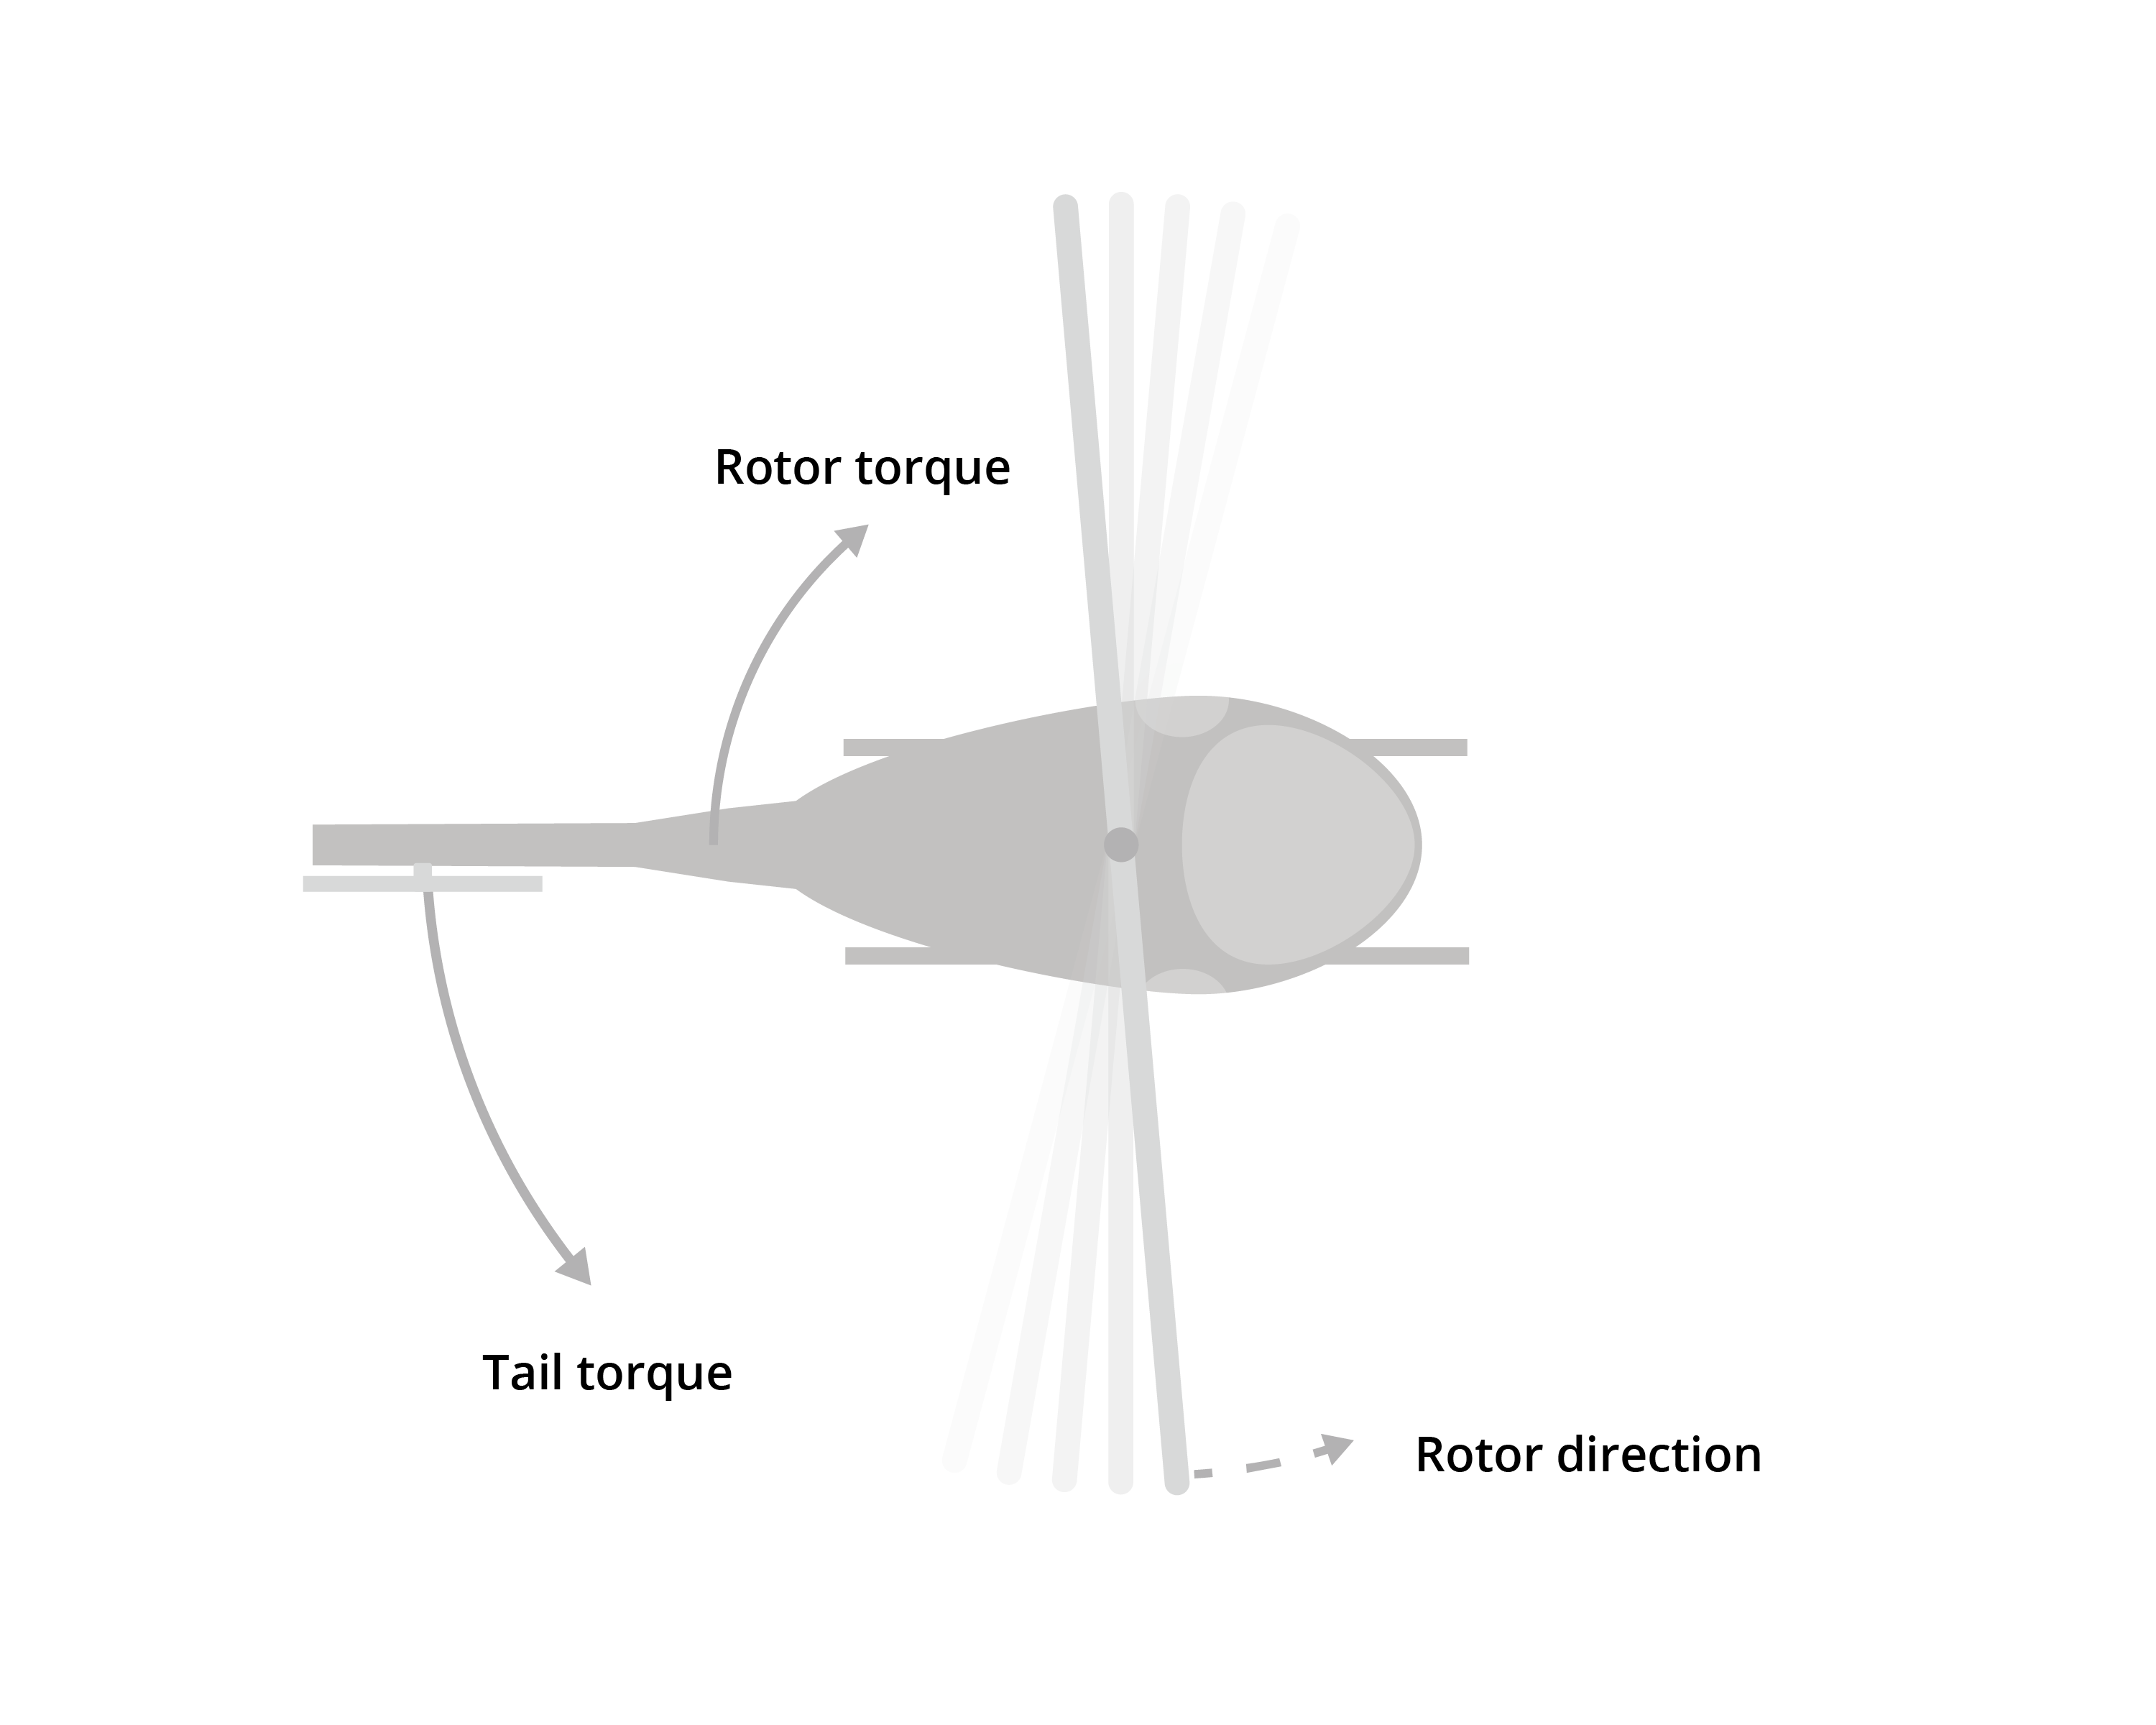
\includegraphics[width=.75\textwidth]{torque.png}


Sequence: Rotor/Tail, Show how the tail rotor works, then show how the control works for the main rotor

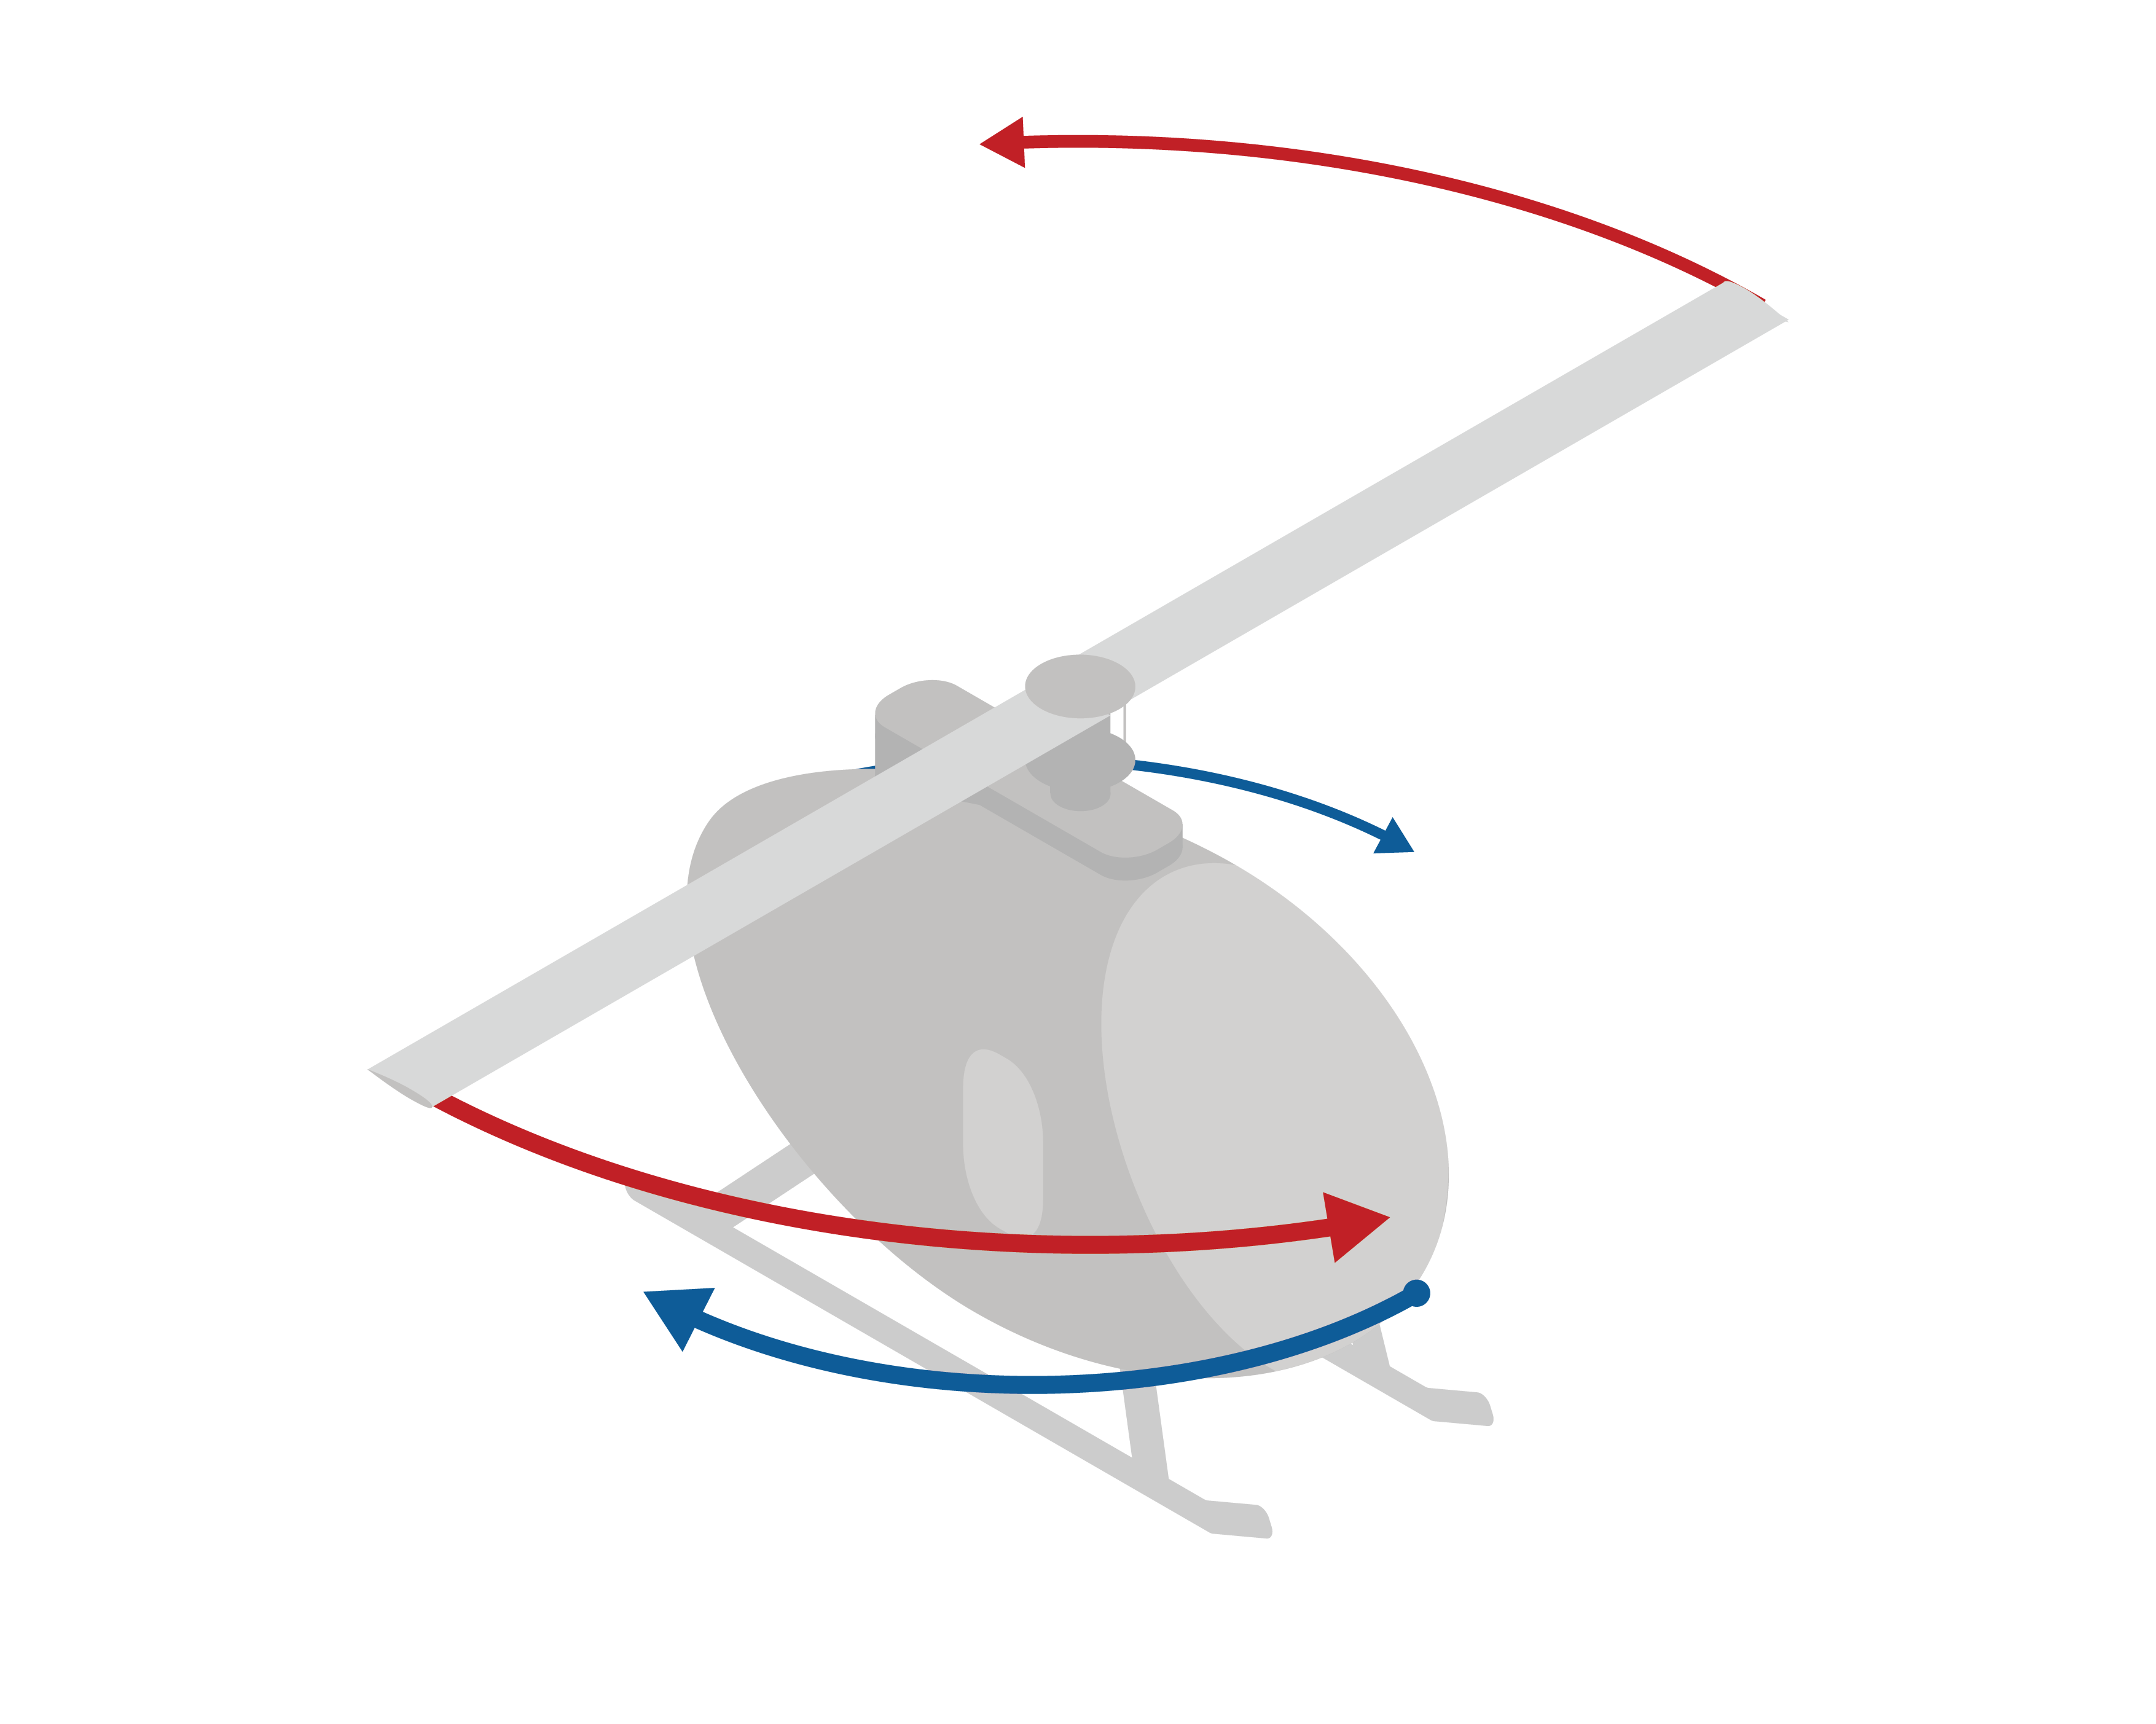
\includegraphics[width=.75\textwidth]{tailless2.png}

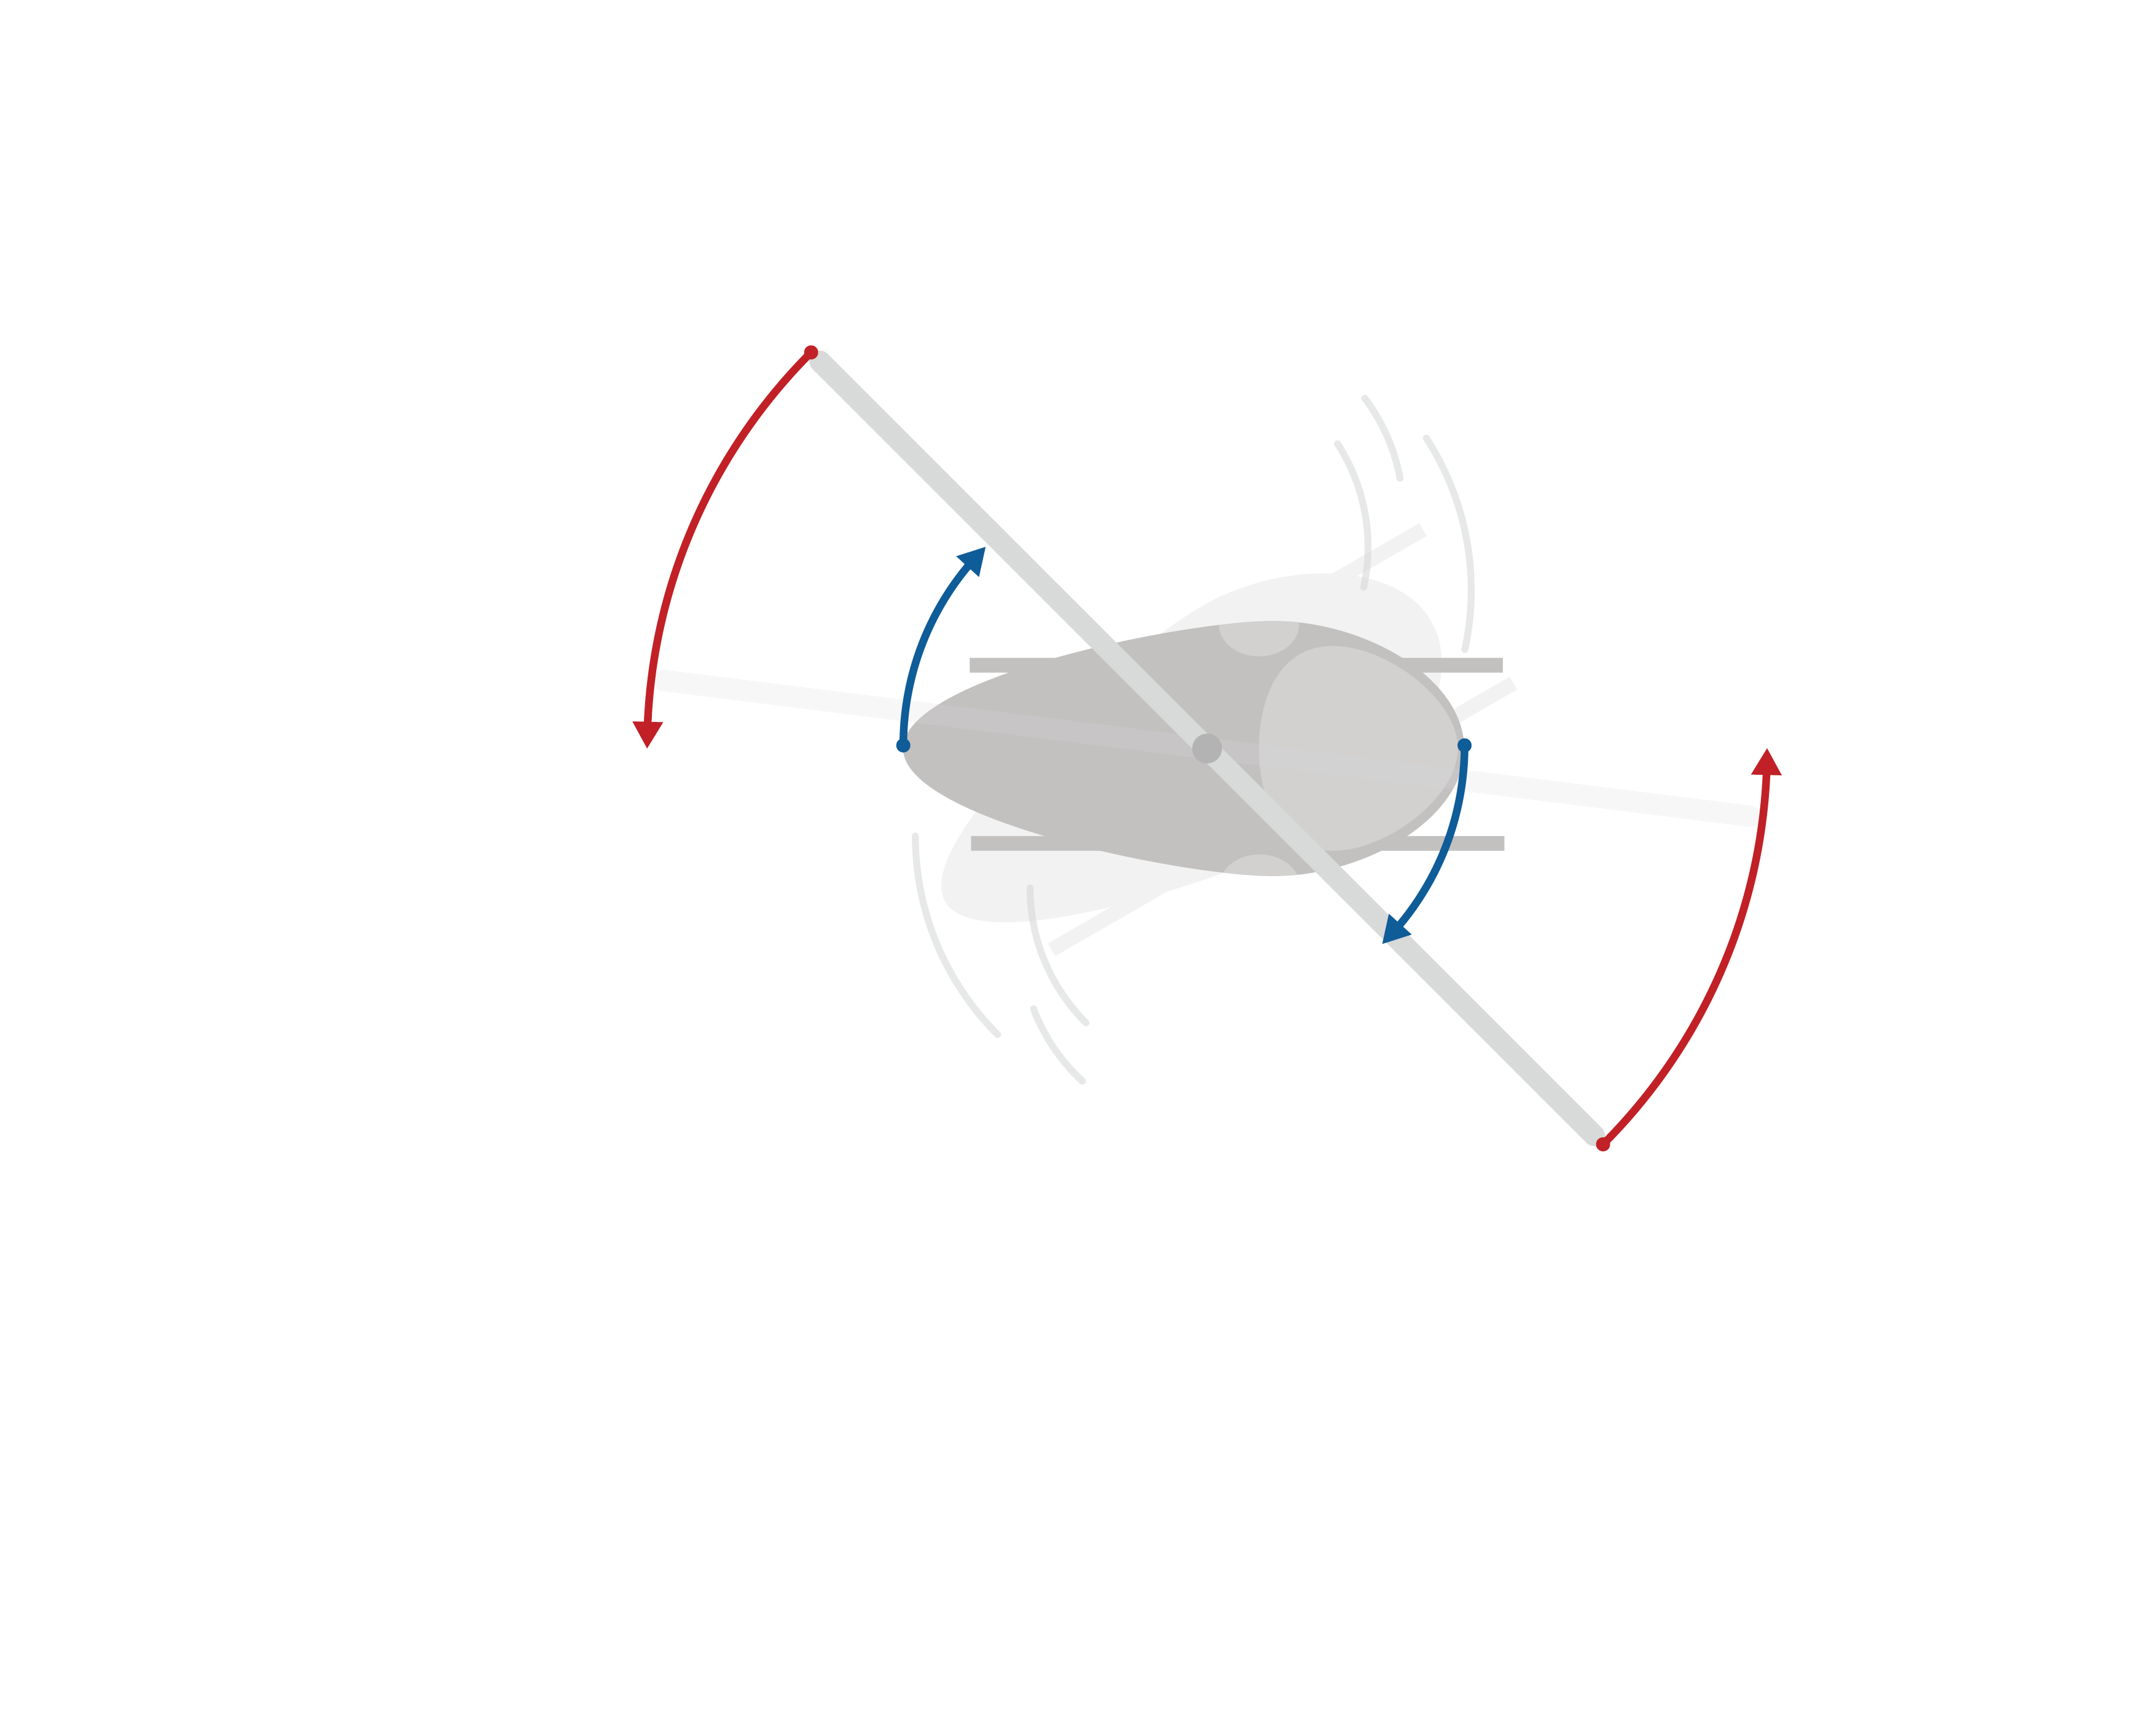
\includegraphics[width=.75\textwidth]{tailless1.png}

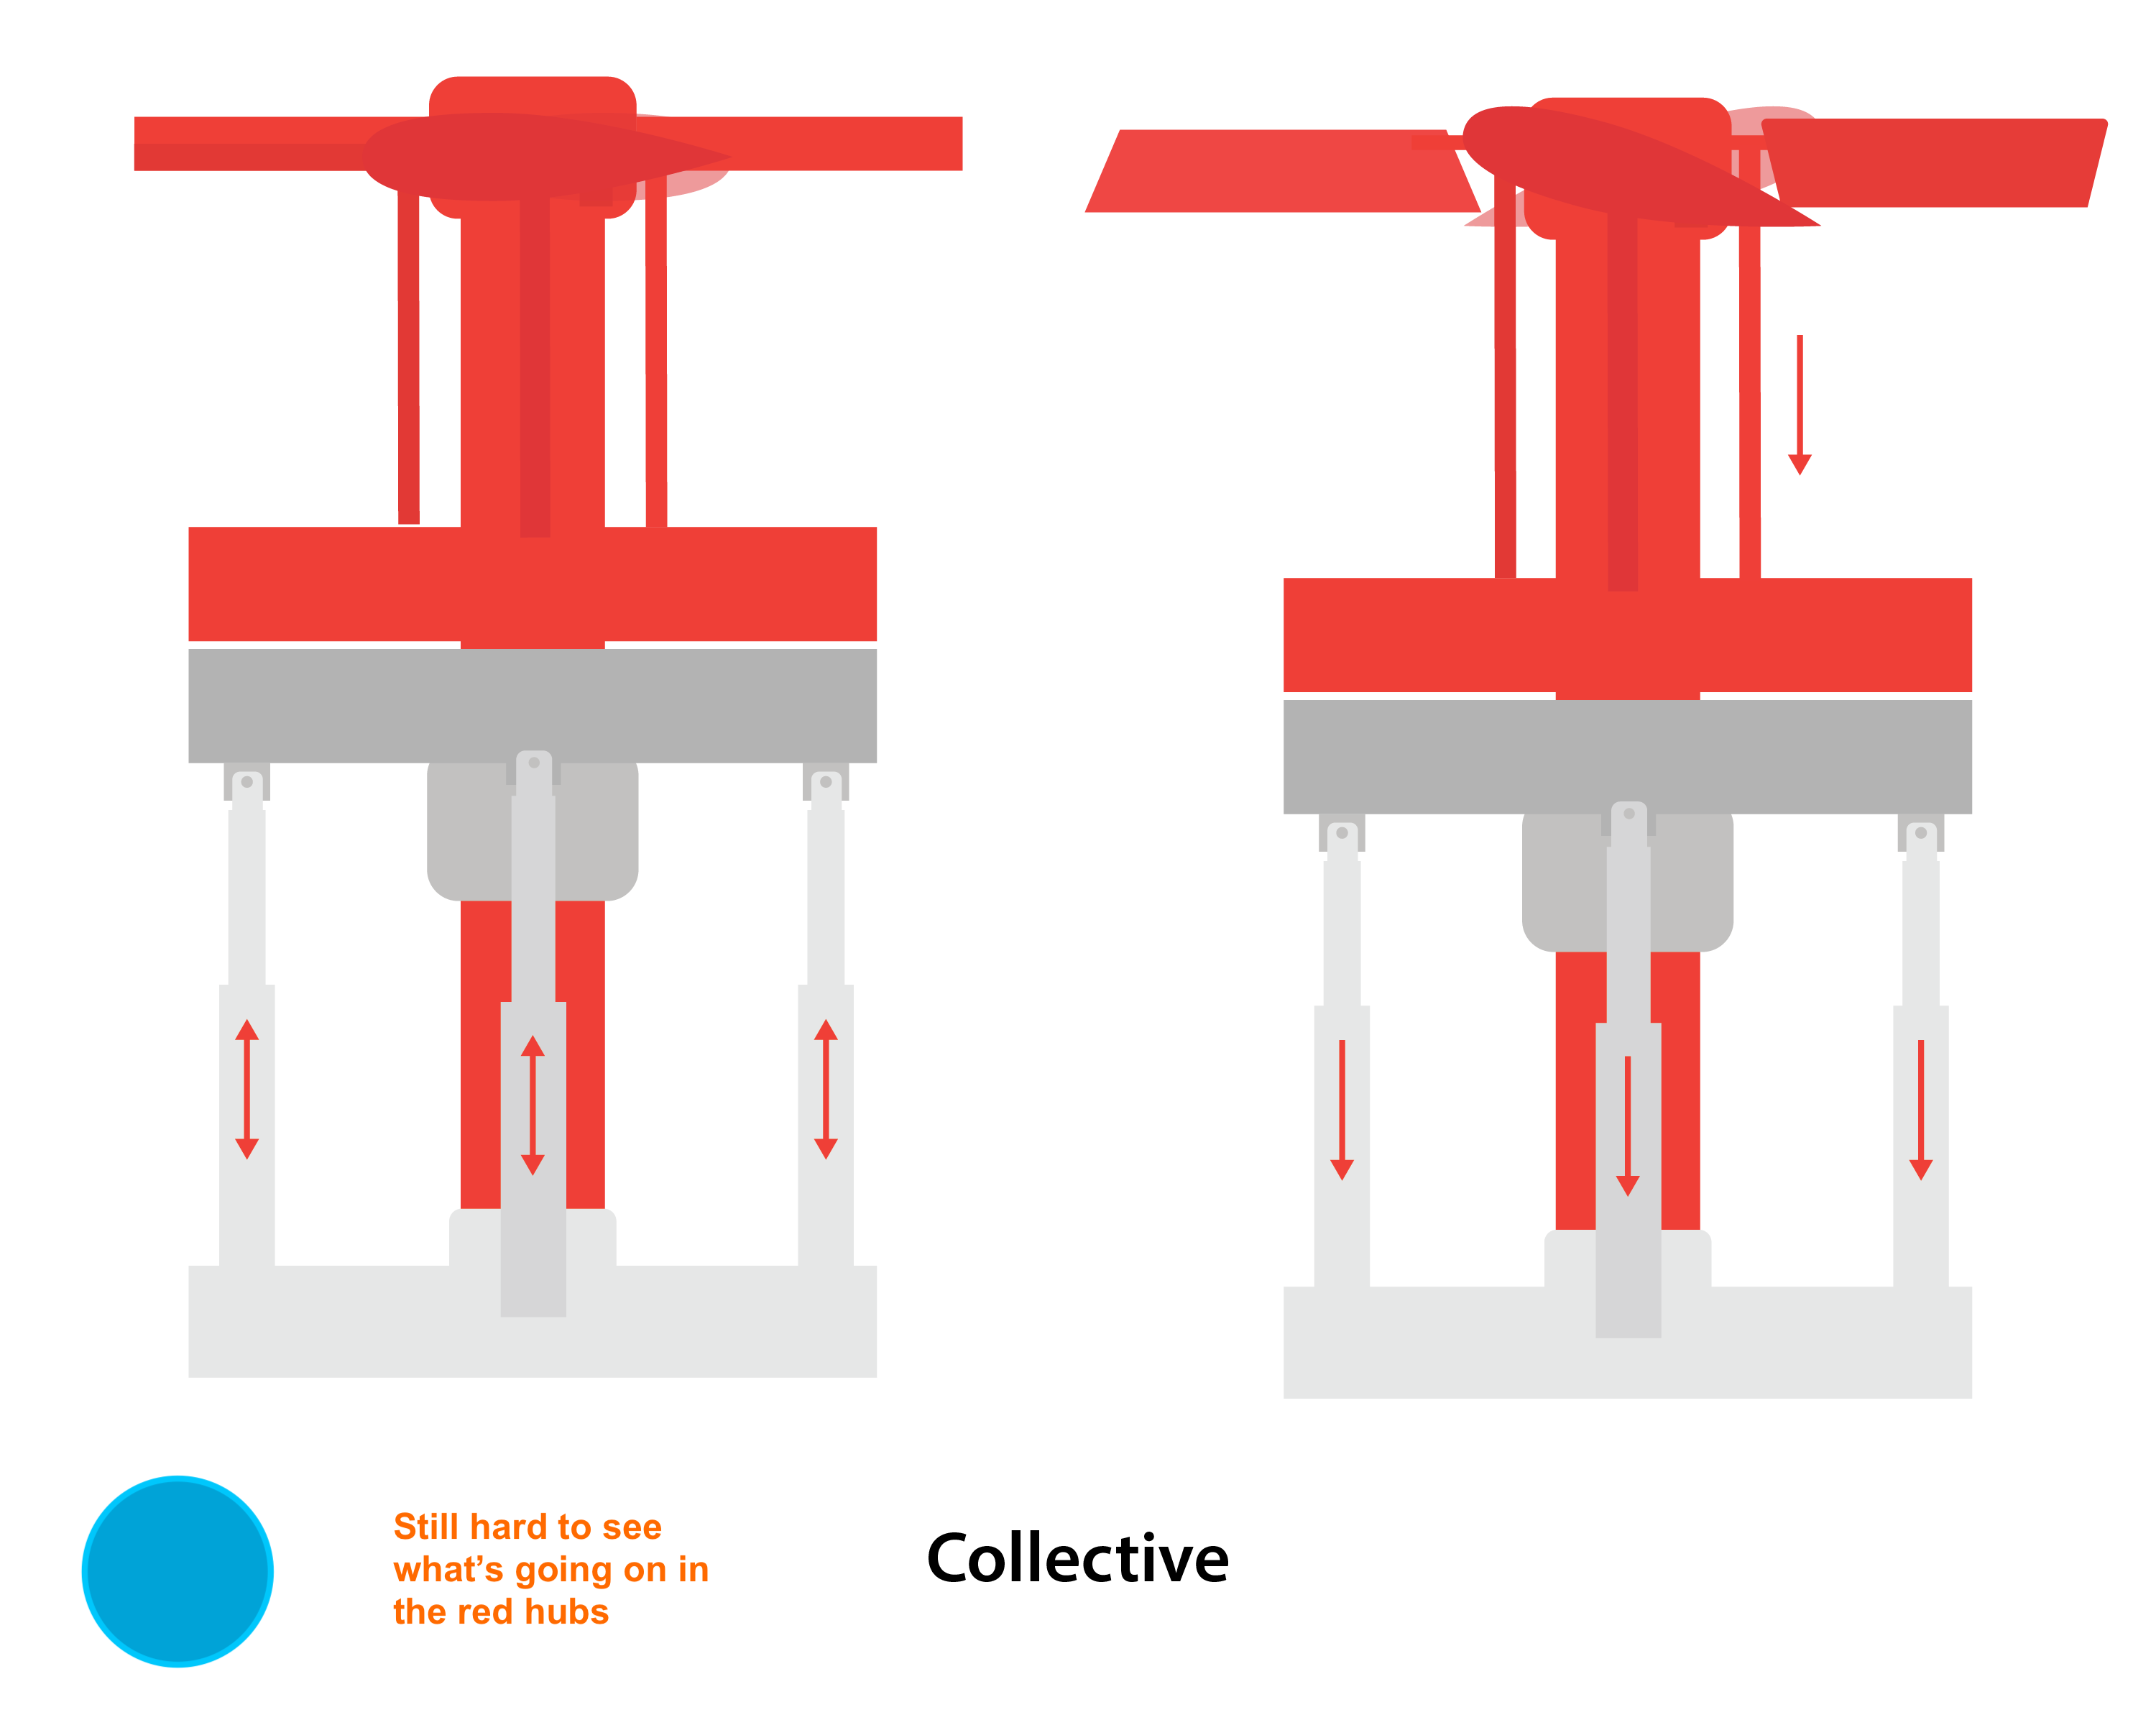
\includegraphics[width=.75\textwidth]{collectiveQuad.png}

